\section{Metamodel for  existing notations and the transformations from them to SACM}
\label{sec:mapping}
SACM is designed to support existing safety notations such as GSN and CAE. 
In previous sections, we briefly demonstrated the usage of SACM elements by comparing them with GSN notations. 
In this section, we provide a GSN metamodel and a CAE metamodel that are compliant to SACM. 
We also discuss the transformation from GSN and CAE to SACM.

\subsection{The GSN Metamodel and the inteoperability from GSN to SACM}
As previously discussed, SACM provides a richer set of features compared to GSN, which includes the ability to standardise evidential and informational artifacts in the models, the ability to standardise controlled vocabularies (expressions and terminologies), as well as modular organisation and integration of artifacts and terminologies. 
In general, creating a metamodel for GSN is a simple task, for there are only several concepts that GSN captures. 
However, it is ideal to create the GSN metamodel by extending SACM elements, so that not only can the GSN metamodel inherit features provided by SACM, but it also makes the interoperability from GSN to SACM easier. 

\begin{figure}
	\centering
	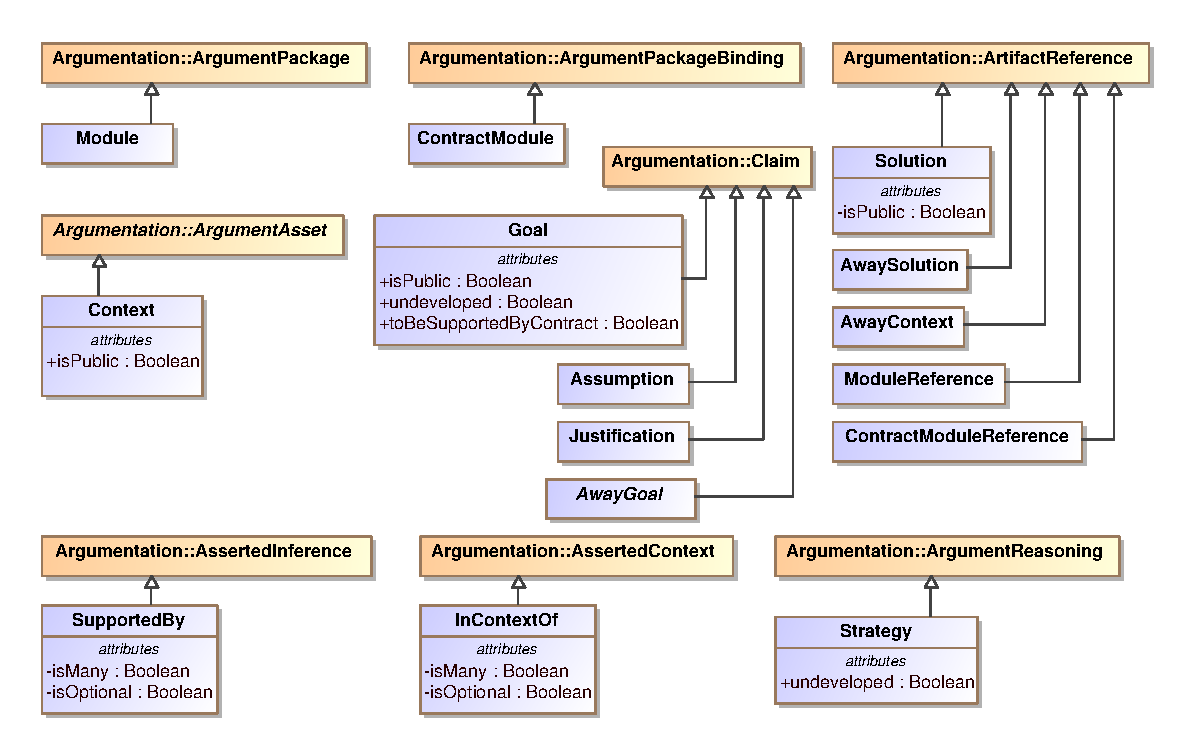
\includegraphics[width=1\linewidth]{GSN.eps}
	\caption{SACM compliant GSN metamodel.}
	\label{fig:gsnMetamodel}
\end{figure}

Our version of the GSN metamodel is shown in Figure~\ref{fig:gsnMetamodel}\footnote{All GSN elements are rendered in blue for readability.}. 
In GSN, argumentations are organised in \textit{Module}s, which is made as a sub-type of \textit{ArgumentPackage} in SACM; \textit{ContractMoudle} are essentially contracts that bind \textit{Module}s together, thus it is a sub-type of \textit{ArgumentPackageBinding}. 

Elements \textit{Goal}, \textit{Assumption}, \textit{Justification} and \textit{AwayGoal} are made sub-types of \textit{Claim} in SACM. 
A \textit{Goal} can be \textit{uninstantiated}, which basically means it is abstract, this is captured by the \textit{+isAbstract} feature in SACM's \textit{SACMElement} class. 
A \textit{Goal} can be \textit{public}, which is deprecated in SACM, a \textit{Goal} can also be \textit{undeveloped} and \textit{toBeSupportedByContract}, which are captured individually. 

Elements \textit{Solution}, \textit{AwaySolution}, \textit{AwayContext}, \textit{ModuleReference} and \textit{ContractModuleReference} are sub-types of \textit{ArtifactReference} in SACM as they refer to artefacts that contain information they represent. 
\textit{Context} is a slightly complicated concept, as it can either be a statement stating the context of a \textit{Claim}, or it can refer to contextual information stored in an artefact. 
Thus, \textit{Context} is made a sub-type of \textit{ArgumentAsset}. 

\textit{SupportedBy} is made a sub-type of \textit{AssertedInference} and \textit{InContextOf} is made a sub-type of \textit{AssertedContext}. 
\textit{Strategy} is made a sub-type of \textit{ArgumentReasoning} for it explains the intention of an \textit{AssertedRelationship}.

The way that the GSN metamodel is created makes it inherently compatible with SACM, so that it can be used as an \textit{ArgumentPackage}, organised in an \textit{AssuranceCasePackage}, with its supporting artefacts organised in \textit{ArtifactPackage}s and controlled vocabularies organised in \textit{TerminologyPckage}s. 

To enable interoperability from GSN to SACM, we provide a model-to-model transformation\footnote{Available at: \url{https://github.com/wrwei/MDERE/blob/master/technical}} defined using the Epsilon Transformation Language (ETL) \cite{kolovos2008epsilon}. 
Most of the transformation is straight forward - instances of the GSN elements are transformed into instances of the SACM elements that the GSN elements extend. 
There is one exception: the transformation from \textit{Strategy} to \textit{ArgumentReasoning}. As discussed in Section~\ref{sec:relationships}, an \textit{ArgumentReasoning} is associated to an \textit{AssertedRelationship}, but in GSN, a \textit{Strategy} acts as a node in a goal structure. 
This requires analysis to be performed during the transformation, which is shown in Algorithm~\ref{alg:s2ar}.
\begin{algorithm}[ht!]
	{
		\fontsize{9}{10}
		\selectfont
		\SetAlgoLined\DontPrintSemicolon
		\SetKwFunction{getUpperLevelSupportedBy}{strategy}
		\SetKwFunction{getLowerLevelSupportedBy}{strategy}
		\SetKwFunction{createModelElement}{createModelElement}
		\SetKwFunction{getCachedModelElement}{getCachedModelElement}
		\SetKwFunction{setFeatureValue}{setFeatureValue}
		\SetKwFunction{setAttributeValue}{setAttributeValue}
		\SetKwFunction{handleObjectAttributes}{handleObjectAttributes}
		\SetKwFunction{handleFeature}{handleFeature}
		
		\SetKwFunction{shouldHandleFeature}{shouldHandleFeature}
		
		\SetKwProg{Procedure}{Procedure}{}{}
		
		\Let strategy = \textit{Strategy} to be transformed;\\
		\Let argumentReasoning = new \textit{ArgumentReasoning};\\
		
		argumentReasoning.name = strategy.name.equivalent();\\
		argumentReasoning.description = strategy.description.equivalent();\\
		\If {strategy.uninstantiated == true} {
			argumentReasoning.isAbstract = true;
		}
		%		\Let supportedByToSolution = all \textit{SupportedBy}s from \textit{outgoingSupportedBy} \\
		%		that connects to a \textit{Solution};\\
		%		\If{supportedByToSolution is not empty}{
		%			\Let assertedEvidence = new \textit{AssertedEvidence};\\
		%			assertedEvidence.target = incomingSupportedBy.source;\\
		%			\For{supportedBy in supportedByToSolution}{
		%				assertedEvidence.source.add(supportedBy.target);\\
		%			}
		%		}
		\Let incomingSupportedBy = the incoming \textit{SupportedBy} to \textit{strategy};\\
		\Let outgoingSupportedBys = all outgoing \textit{SupportedBy}s from \textit{strategy};\\
		\Let supportedByFromGoal = \textit{Goal} from \textit{incomingSupportedBy}\\
		\Let supportedByToGoals = all \textit{Goal}s from \textit{outgoingSupportedBys} that connects to \textit{strategy};\\
		\If{supportedByToGoal is not empty}{
			\Let assertedInference = new \textit{AssertedInference};\\
			assertedInference.target = supportedByFromGoal.equivalent();\\
			\For{goal in supportedByToGoals}{
				assertedInference.source.add(goal.equivalent());\\
			}
		}
	}
	\
	\caption{Transforming Rule Strategy2ArgumentReasoning}
	\label{alg:s2ar}
\end{algorithm}

Algorithm~\ref{alg:s2ar} defines the transformation rule \textit{Strategy2ArgumentReasong}. 
Line 1 retrieves the \textit{Strategy} to be transformed;
Line 2 creates a new \textit{ArgumentReasoning};
Line 3 and 4 transform the \textit{name} and \textit{description} of the \textit{Strategy} to the \textit{ArgumentReasoning} (the equivalent() operation in ETL divert control to corresponding transformation rules that transform \textit{Name} to \textit{Name}, and returns the transformed model element).
Line 5 checks if the \textit{Strategy} is uninstantiated, and then in line 6, make the \textit{ArgumentReasoning} \textit{abstract}.
Line 8 retrieves the incoming \textit{SupportedBy}  for the \textit{Strategy}.
Line 9 retrieves all outgoing \textit{SupportedBy} for the \textit{Strategy} (In GSN, the flow of an argument goes from top to bottom. Thus, for a \textit{Strategy}, there is one incoming \textit{SupportedBy} and many outgoing \textit{SupportedBy}s).
Line 10 retrieves the \textit{Goal} from the incoming \textit{SupportedBy}.
Line 11 retrieves the \textit{Goal}s from the outgoing \textit{SupportedBy}s. 
Then, in line 13 an \textit{AssertedInference} is created. 
It is worth noting that in SACM, the inference flows from bottom to top. Thus the source and target of the \textit{AssertedInference} are the transformed counterparts of \textit{supportedByToGoals} in line 11 and the transformed counterparts of \textit{supportedByFromGoal} in line 10, respectively.

It is worth noting that some developers use \textit{Solutions} to directly support \textit{Strategy}. 
This is forbidden in the GSN standard (permitted SupportedBy connections are: \textit{Goal}-to-\textit{Goal}, \textit{Goal}-to-\textit{Strategy}, \textit{Goal}-to-\textit{Solution} and \textit{Strategy}-to-\textit{Goal}). 
This is one of the reasons why model-based assurance case is desired - automated model validation can be performed to check the well-formedness of assurance cases.

\subsection{The CAE metamodel and the interoprability from CAE to SACM}
Claims-Arguments-Evidence (CAE) \cite{bishop2000methodology} is another widely used notation to construct safety arguments. Concepts in CAE are similar to those in GSN. 
There has not been an official metamodel defined for CAE. Thus, we provide our own version of CAE that extends SACM, shown in Figure~\ref{fig:caeMetamodel}\footnote{All CAE elements are rendered in blue for readability.}.


\begin{figure}
	\centering
	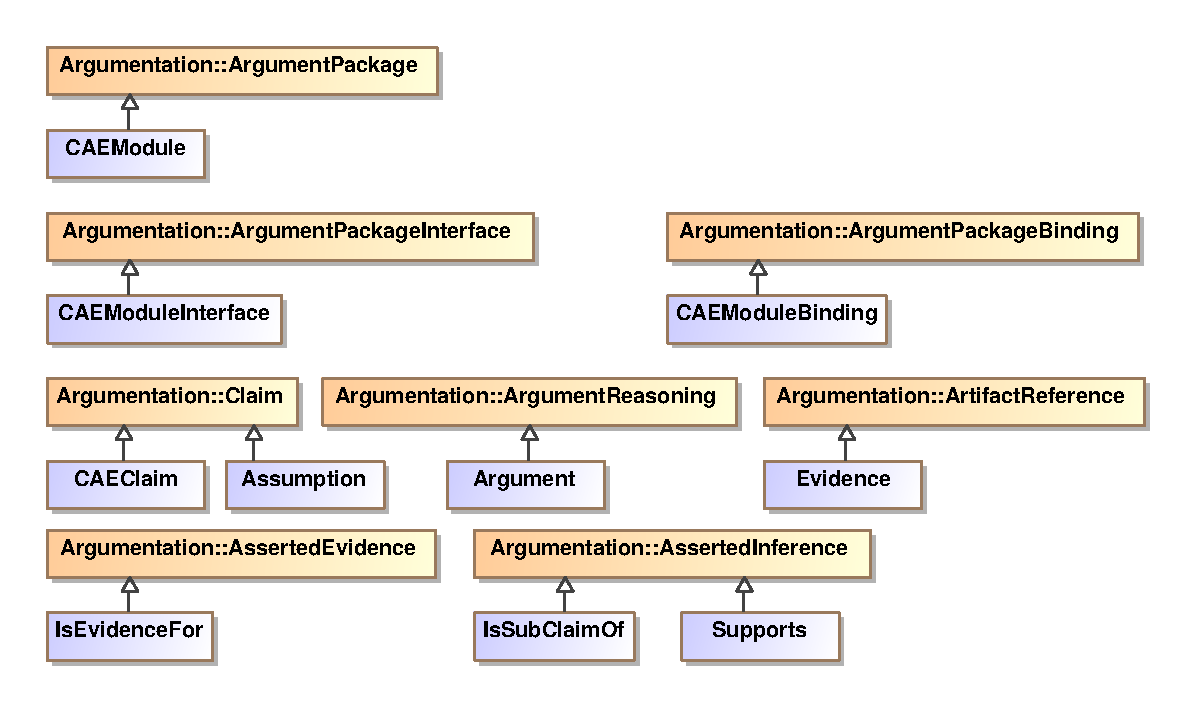
\includegraphics[width=1\linewidth]{CAE.eps}
	\caption{SACM compliant CAE metamodel.}
	\label{fig:caeMetamodel}
\end{figure}

CAE does not support modularity.
However, SACM is highly modular.
Therefore, we introduced three new concepts in CAE, \textit{CAEModule}, \textit{CAEModuleInterface} and \textit{CAEModuleBinding}, which extend \textit{ArgumentPackage}, \textit{ArgumentPackageInterface} and \textit{ArgumentPackageBiding} respectively.
In CAE, there is a notion of \textit{Claim}, which is semantically identical to \textit{Claim} in SACM. 
We therefore create a \textit{CAEClaim} element that extends \textit{Claim} in SACM. 
The reason for this redundancy is that we want the CAE metamodel to be non-invasive to SACM. 
The \textit{Argument} elements in CAE provide a description of the argument approach, which is functionally equivalent to \textit{ArgumentReasoning}, thus it is made a sub-type of \textit{ArgumentReasoning}.
\textit{Evidence} is made a sub-type of \textit{ArtifactReference} because it is a reference to evidential materials. 
In CAE, there is a notion of \textit{Assumption}, which is made a sub-type of \textit{Claim}. 

In CAE, there are three types of relationships, the \textit{IsEvidenceFor} connects \textit{Evidence} with \textit{Claim}s, thus is made a sub-type of \textit{AssertedEvidence}; the \textit{IsSubClaimOf} relationship connects sub-\textit{Claim}s to \textit{Claim} and is made a sub-type of \textit{AssertedInference}; the \textit{Supports} relationship connects \textit{Argument}s to \textit{Claim} and is also made a sub-type of \textit{AssertedInference}. 
Since there is no notion of modules in CAE, the argumentation is contained in \textit{ArgumentPackage}s inherited from SACM.

The transformation from CAE to SACM is similar to the transformation from GSN to SACM (which is also implemented in Epsilon Transformation Language), with the same issue that \textit{Argument} needs to be \textit{ArgumentReasoning}. 
The detailed transformation is made publicly available\footnote{Available at: \url{https://github.com/wrwei/MDERE/blob/master/technical}}.



